\documentclass[12pt,fleqn,handout]{beamer}


\xdefinecolor{lavendar}{rgb}{0.8,0.6,1}
\xdefinecolor{olive}{cmyk}{0.64,0,0.95,0.4}
%\xdefinecolor{olive}{cmyk}{1,0,0,0}
\xdefinecolor{mag}{cmyk}{0.1,1,0,0.2}
\xdefinecolor{lblue}{rgb}{0,0,1.5}
\xdefinecolor{lred}{rgb}{1,0,0}
\xdefinecolor{mine}{cmyk}{1,0,0.2,0}
\xdefinecolor{bluel}{cmyk}{0.1,0,0.9,0.4}

\usepackage{amsmath,amssymb,dsfont,mathrsfs}
\usepackage{tikz,pgflibraryplotmarks}
\usepackage{multimedia}
\usepackage{wasysym}
\usepackage{rotating}
\usepackage{algorithm,algorithmic}
\usepackage{graphicx} % more modern
\usepackage{subfigure}
\usepackage{booktabs}

\usepackage{pgfplots}
\usepackage{verbatim}

\usepackage{setspace}
\newlength\iwidth
\newlength\iheight

\newcommand\makebeamertitle{\frame{\maketitle}}%
\graphicspath{{./images/}}
\setbeamertemplate{navigation symbols}{}
\addtobeamertemplate{navigation symbols}{}{%
    \usebeamerfont{footline}%
    \usebeamercolor[fg]{footline}%
	\insertshorttitle
    \;--
    \insertframenumber
}

\newcommand{\sectionstart}{
	\only<beamer>{
 	\begin{frame}% (fold)
 		\begin{centering}\Huge \insertsection \par\end{centering}
 	\end{frame}% frame the_application (end)
	}
 }


% make bibliography entries smaller
\usepackage{natbib}
\setbeamertemplate{bibliography item}{[\theenumiv]}
\renewcommand\bibfont{\scriptsize}
\setbeamertemplate{frametitle continuation}[from second]
\newcommand{\tcr}{\textcolor{red}}
\newcommand{\tcrd}{\textcolor{red}}
\newcommand{\tcb}{\textcolor{bluel}}
\newcommand{\tcm}{\textcolor{mag}}
\newcommand{\tcg}{\textcolor{olive}}

\newcommand{\R}{\mathbb{R}}
\newcommand{\C}{\mathbb{C}}

% bold lower-case for vectors
\newcommand{\bfa}{{\bf a}}
\newcommand{\bfb}{{\bf b}}
\newcommand{\bfc}{{\bf c}}
\newcommand{\bfs}{{\bf s}}
\newcommand{\bfm}{{\bf m}}
\newcommand{\bfd}{{\bf d}}
\newcommand{\bfe}{{\bf e}}
\newcommand{\bfu}{{\bf u}}
\newcommand{\bfy}{{\bf y}}
\newcommand{\bfx}{{\bf x}}
\newcommand{\bfh}{{\bf h}}
\newcommand{\bfw}{{\bf w}}
\newcommand{\bfv}{{\bf v}}
\newcommand{\bfr}{{\bf r}}
\newcommand{\bfz}{{\bf z}}
\newcommand{\bfp}{{\bf p}}


% bold upper-case for linear operators
\newcommand{\bfA}{{\bf A}}
\newcommand{\bfB}{{\bf B}}
\newcommand{\bfZ}{{\bf Z}}
\newcommand{\bfM}{{\bf M}}
\newcommand{\bfC}{{\bf C}}
\newcommand{\bfD}{{\bf D}}
\newcommand{\bfQ}{{\bf Q}}
\newcommand{\bfJ}{{\bf J}}
\newcommand{\bfG}{{\bf G}}
\newcommand{\bfI}{{\bf I}}
\newcommand{\bfP}{{\bf P}}
\newcommand{\bfK}{{\bf K}}
\newcommand{\bfY}{{\bf Y}}
\newcommand{\bfW}{{\bf W}}
\newcommand{\bfR}{{\bf R}}
\newcommand{\bfL}{{\bf L}}
\newcommand{\bfF}{{\bf F}}
\newcommand{\bfT}{{\bf T}}
\newcommand{\bfS}{{\bf S}}
\newcommand{\bfX}{{\bf X}}
\newcommand{\bfU}{{\bf U}}
\newcommand{\bfV}{{\bf V}}
\newcommand{\bfH}{{\bf H}}


\newcommand{\calF}{\mathcal{F}}



\newcommand{\hf}{{\frac 12}}
\newcommand{\bftheta}{{\boldsymbol \theta}}
\newcommand{\bfxi}{{\boldsymbol \xi}}

\newcommand{\bfLambda}{{\boldsymbol \Lambda}}
\newcommand{\bfSigma}{{\boldsymbol \Sigma}}
\newcommand{\bfepsilon}{{\boldsymbol \epsilon}}

\newcommand{\E}{\vec E}
\newcommand{\B}{\vec B}

\newcommand{\vu}{  {\vec {\bf u}}}

\newcommand{\grad}{  {\vec {\bf \nabla}}}

\newcommand{\lfrownie}{\textcolor{red}{\large{\frownie}}}
\newcommand{\lsmiley}{\textcolor{green}{\large{\smiley}}}

\newcommand{\curl}{\ensuremath{\nabla\times\,}}
\renewcommand{\div}{\nabla\cdot\,}
\newcommand{\divh}{\nabla_h\cdot\,}
\renewcommand{\grad}{\ensuremath{\nabla}}

\DeclareMathOperator*{\argmin}{arg\,min}
\date{}

\title[CNN+PDE]{Convolutional Neural Networks and PDEs}
\subtitle{Numerical Methods for Deep Learning}

\begin{document}

\makebeamertitle

\begin{frame}[fragile]\frametitle{Recall - Deep Network}

$$ \bfY_{j+1} = \bfP_j\bfY_j +  \sigma(\bfK_j \bfY_j + b_j) $$

\bigskip
\pause

Problems/Challenges

\begin{itemize}
\item
The state can grow (explosion) $\Rightarrow$ $\bfY_N$  very sensitive to $\bfY_0$ and $\bfK_j$
(exploding gradients)
\pause
\item
The state can go to $0$ $\Rightarrow$ $\bfY_N$ independent to  $\bfY_0$ and to the $\bfK_j$'s
(vanishing gradients)
\item
In both cases the optimization can fail
\end{itemize}

\end{frame}

\begin{frame}
	\frametitle{Today: Deep Convolutional Neural Networks}
	
	Deep network with convolution operators parameterized by stencils. Common
	$$ \bfY_{j+1} = \bfP_j\bfY_j +  h \bfK_{j,2}\sigma(\bfK_{j,1} \bfY_j + b_j) $$
	
	\bigskip
	\pause
	
	Motivation for second convolution?
	\begin{itemize}
		\item approximation properties of double layer
		\item if $\sigma(x)=\max(x,0)$ entries in $\bfY$ can only grow.
	\end{itemize}
	
	\bigskip
	\pause
	
	Learning tasks:
	\begin{itemize}
		\item image classification
		\item semantic segmentation
	\end{itemize}
	
	
	
\end{frame}

\begin{frame}\frametitle{Convolutions and PDEs}

Let $\bfy$ be 1D grid function, $\bfy \leftrightarrow y$ ($n$ cells of width $h_x=1/n$)

\begin{align*}
K(\theta)\bfy & = [\theta_1\; \theta_2\; \theta_3] * \bfy  \\
 & =\left(\frac{\beta_1}{4} [1\;\; 2\;\; 1]  + \frac{\beta_2}{2h_x} [-1\;\; 0 \;\; 1] + \frac{\beta_3}{h_x^2}[-1\;\; 2 -1] \right) * \bfy
\end{align*}

\pause
Relation between $\beta$ and $\theta$ given by
$$
	\underbrace{
	\left( 
		\begin{array}{rrr}
			1/4 & -1/(2h_x) & -1/h_x^2 \\
			1/2 & 0            & 2/h_x^2  \\
			1/4 & 1/(2h_x)  & -1/h_x^2
		\end{array}
	\right)}_{=\bfA(h_x)}
	\left( 
		\begin{array}{r}
			\beta_1 \\ 
			\beta_2 \\
			\beta_3
		\end{array}
	\right)
	=
	\left( 
		\begin{array}{r}
			\theta_1 \\ 
			\theta_2 \\
			\theta_3
		\end{array}
	\right).
$$

\bigskip
\pause

In the limit $h_x \to 0$ this gives
$$
	K(\theta(t)) = \beta_1(t) + \beta_2(t) \partial_x + \beta_3(t) \partial_x^2.
$$
\pause

\end{frame}

\begin{frame}
	\frametitle{Scaling Convolution Operators: Rediscretization}
	
	Let $\bfy_c$ and $\bfy_f$ be 1D grid functions $\bfy \leftrightarrow y$ (grid: $n_c=n$ and $n_f=2n$ cells of width $h_c=1/n_c$ and $h_f = 1/n_f$, respectively)
	
	\bigskip
	\pause
	
	Ex: Let $y(x) = (cos(2 \pi x^4))+x-0.8(x-0.5)^2$, $n = 8$, and
	$$
		\theta_{\rm coarse} = (-67,  129, -59)^\top.
	$$
	Find corresponding kernel, $\theta_{\rm fine}$  on fine mesh.
	
	\bigskip
	\pause
	
	Strategy:
	\begin{enumerate}
		\item setup $\bfA(h_c)$ and compute $\beta$
		\item setup $\bfA(h_f)$ and compute $\theta_{\rm fine}$
	\end{enumerate}
	
	\bigskip

	\begin{center}
		\texttt{E15CoarseToFineConv1D.m}
	\end{center}
	
\end{frame}

\begin{frame}
	\frametitle{Convolution and PDEs - 2D Case}
	
	Similar arguments apply in two and more dimensions. Let $\theta\in\R^{3\times 3}$ be a given stencil then
	\begin{align*}
		K(\theta) =&  \beta_1  + \beta_2 \partial_x + \beta_3 \partial_y + \beta_4 \partial_{xy} + \beta_5 \partial_{xx} \\
		& + \beta_6 \partial_{yy} + \beta_7 \partial_{x^2y} + \beta_8 \partial_{xy^2} + \beta_9 \partial_{x^2y^2}
	\end{align*}
	How to get the coefficients? Let $h_x>0$ pixel size, use 
	$$
		\left(
		\begin{array}{rrr|rrr|rrr}
			1 & -1 & -1 &  1 &  1 & -1 & -1 & -1 & -1\\ 
			2 & -2 &  0 &  2 & -2 &  0 &  2 &  0 &  2\\ 
			1 & -1 &  1 &  1 &  1 &  1 & -1 &  1 & -1\\ 
			2 &  0 & -2 & -2 &  2 &  0 &  0 &  2 &  2\\ 
			4 &  0 &  0 & -4 & -4 &  0 &  0 &  0 & -4\\ 
			2 &  0 &  2 & -2 & -2 &  0 &  0 & -2 &  2\\ 
			1 &  1 & -1 &  1 &  1 &  1 &  1 & -1 & -1\\ 
			2 &  2 &  0 &  2 & -2 &  0 & -2 &  0 &  2\\ 
			1 &  1 &  1 &  1 &  1 & -1 &  1 &  1 & -1\\ 
		\end{array}
		\right)
		\cdot {\rm diag}
		\begin{pmatrix}
			1/16.  \\
			1/6h_x \\
			1/6h_x \\
			1/4h^2 \\
			1/4h^2 \\
			1/h^2  \\
			1/2h^3 \\
			1/2h^3 \\
			1/2h^3
		\end{pmatrix}
	$$
	
\end{frame}


\begin{frame}\frametitle{Algebraic Prolongation of Convolution Kernels}

\begin{columns}
	\column{.55\textwidth}
	\begin{equation*}
		\bfK_H = \bfR \bfK_h \bfP,
	\end{equation*}
	where
	\begin{itemize}
		\item $\bfK_h$ fine mesh operator (given)
		\item $\bfR$ restriction (e.g., averaging)
		\item $\bfP$ prolongation (e.g., interpolation)
	\end{itemize}
	
	
	\pause
 	Remarks:
\begin{itemize}
	\item Galerkin: $\bfR = \gamma\bfP^\top$
	\item Coarse $\rightarrow$ Fine: unique if kernel size constant.
	\item only small linear solve required 
\end{itemize}


	\column{.5\textwidth}
	
	\pause
	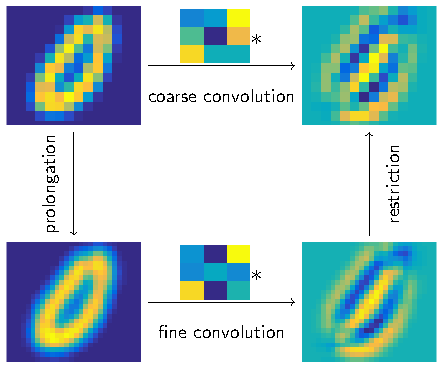
\includegraphics[width=55mm]{convDiagram}
	
	
\end{columns}
\end{frame}


 \begin{frame}
 	\frametitle{Scaling Convolution Operators: Algebraic}

 Let $n_c=3$, $n_f=6$ (see \texttt{E15CoarseToFineConv1D.m})

 	Prolongation and restriction
 	$$
 		\bfP = \left(
 			\begin{array}{rrr}
 				1 &  \\
 				3/4 & 1/4 & \\
 				1/4 & 3/4 & \\
 				    & 3/4 & 1/4\\
 					& 1/4 & 3/4\\
					&    & 1
 			\end{array}
 		\right),
 	$$
	\pause
	$$
		\bfR = \left(
			\begin{array}{rrrrrr}
				1/2 & 1/2 \\
				    &     & 1/2  & 1/2 \\
					&     &     &     & 1/2 & 1/2 \\
			\end{array}
		\right)
	$$
	\pause
	\begin{enumerate}
		\item build $\bfK_H = \bfR \bfK_h \bfD$ for $j$th unit vector as stencil
		\item extract a column associated with interior node
		\item reshape and get patch around node
		\item vectorize and use as one column
	\end{enumerate}


 	\begin{center}
 		
 	\end{center}

 \end{frame}

\begin{frame}
	\frametitle{Stability of Convolutional ResNets}
	
	Residual Neural Network is discretization of 
	$$
		\partial_t \bfy(t) = \bfK_2(t) \sigma\left(\bfK_1(t) \bfy + b(t)\right), \quad \bfy(0)= \bfy_0.
	$$
	\pause
	
	To analyze stability need to look at eigenvalues of 
	$$
		\bfJ(t) = \bfK_2(t) {\rm diag}\left(\sigma'(\bfK_1(t) \bfy + b)\right) \bfK_1(t)
	$$
	Difficult to analyze eigenvalues for general $\bfK_2$ and $\bfK_1$. 
	
	\pause
	
	Easy option: Set $\bfK_2 = - \bfK_1^\top$ (and drop subscript index). Doing so gives:
	$$
		\bfJ_{sym}(t) - \bfK(t)^\top {{\rm diag}\left(\sigma'(\bfK_1(t) \bfy + b)\right)} \bfK(t)
	$$
	symmetric negative definite $\leadsto$ stability if $\partial_t \bfK$ small
	
	\begin{center}
		\texttt{E15ParabolicCNN.m}
	\end{center}
	
\end{frame}

\begin{frame}
	\frametitle{Parabolic CNN}

		In original Residual Net choose $\bfK_2 = - \bfK_1^\top = \bfK^\top$.
		This gives parabolic CNN
		$$
		 \partial_t \bfY_{t} = -\bfK(t)^{\top} \sigma(\bfK(t) \bfY  + \bfb(t)), \quad \bfY(0) = \bfY_0 
		$$
		
	 \pause
	
	\begin{theorem}
	    If $\sigma$ is monotonically non-decreasing, then the forward propagation is stable, i.e., there is a $M>0$ such that
	    \begin{equation*}
	        \|\bfY(T) - \bfY_{\epsilon}(T)\|_F \leq M \|\bfY(0) - \bfY_{\epsilon}(0)\|_F,
	    \end{equation*}
	    where $\bfY$ and $\bfY_{\epsilon}$ are solutions for different initial values.
	\end{theorem}
		
	 	Use forward Euler discretization with $h$ small enough
	 	\begin{equation*}
	 		\bfY_{j+1} = \bfY_{j}-h\bfK_j^{\top} \sigma(\bfK_j \bfY  + \bfb_j), \quad j=0,1,\ldots,N-1
	 	\end{equation*}
	 	Similar to anisotropic diffusion (popular in image processing)~\cite{ChenPock2017}
\end{frame}

\begin{frame}
	\frametitle{Proof: Stability of Parabolic Networks}
	

	% \begin{proof}
	    For ease of notation,  assume no bias.
		We show that 
			    \begin{equation*}
			        \partial_t \|\bfY(t) - \bfY_{\epsilon}(t)\|_F^2 \leq 0.
			    \end{equation*}
		Integrating this over $[0,T]$ yields the stability result.
		
		\pause
	    Why? Note that for all $t \in [0,T]$ taking derivative gives
	    \begin{eqnarray*}
			\left( -\bfK(t)^\top \sigma(\bfK(t) \bfY) + \bfK(t)^\top\sigma(\bfK(t) \bfY_\epsilon),  \bfY- \bfY_{\epsilon}\right)& \pause\\
	         -\left( \sigma(\bfK(t) \bfY) - \sigma(\bfK(t) \bfY_\epsilon),  \bfK(t) (\bfY- \bfY_{\epsilon}) \right)
	        & \leq  0.
	    \end{eqnarray*}
	    Where $(\cdot,\cdot)$ is inner product and the inequality follows from the monotonicity of the activation function.
	% \end{proof}
	
\end{frame}

\begin{frame}
	\frametitle{Relation to Total Variation}
	

	Note that the parabolic network can be seen as a gradient flow for
	$$
		\phi(\bfY) = s(\bfK(t) \bfY(t) + b(t)),
	$$
	where $\sigma(x) = s'(x)$. What is $s$?
	
	\begin{columns}
		\column{.6\textwidth}
	\begin{itemize}
		\item $\sigma = \max(x,0)$: 
		$$
			s(x) = \max(x,0)^2
		$$
		\item $\sigma = \tanh(x)$:
		$$
			s(x) = \log(\exp(x) - \exp(-x))
		$$
		
		For $\bfK(t) = \nabla$, this shows a relation to total variation~\cite{RudinOsherFatemi1992}.
	\end{itemize}
		
		\column{.4\textwidth}
		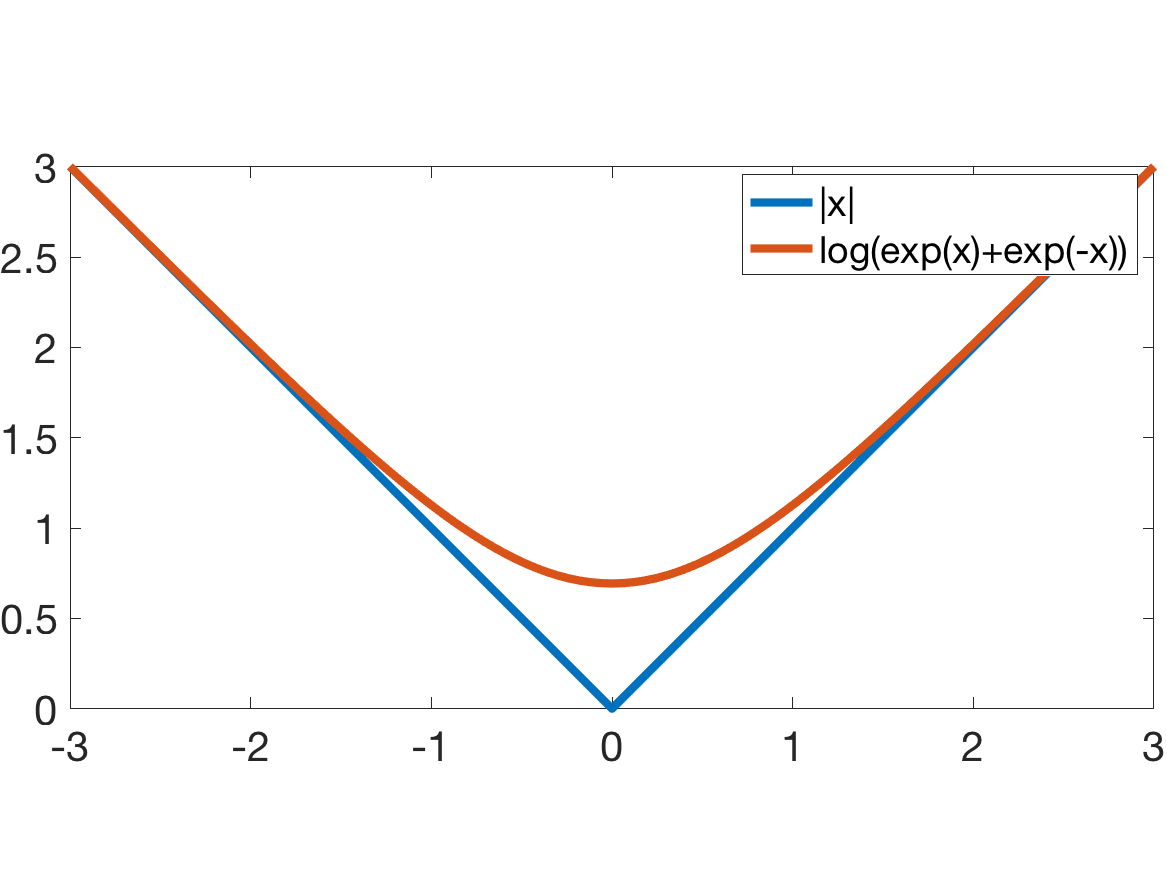
\includegraphics[width=4.5cm]{E15-TV}
		
		\footnotesize thanks to Stanley Osher for providing this example
	\end{columns}
\end{frame}


\begin{frame}[fragile]\frametitle{Normalization}

Goal: Make sure $\|\bfY_j\|$ does not change too much.


\bigskip

\begin{enumerate}
	\item Compute
$$ \bfZ_j = \bfK_j \bfY_j $$

	\item ``Normalize''
$$ \widehat \bfZ_j = N( \bfZ_j) $$

	\item Update
	$$ 
	\bfY_{j+1} = \bfP_j\bfY_j - h \bfK_j^\top  \sigma( \alpha_j  \widehat \bfZ_j + \beta_j), $$
	where $\alpha_j,\beta_j$ are trainable weights.

\end{enumerate}





\bigskip
\bigskip

\begin{center}
How to normalize?	
\end{center}


\end{frame}

\begin{frame}[fragile]\frametitle{Normalization}

\begin{center}
	\begin{tikzpicture}
		\node at (-2,0) {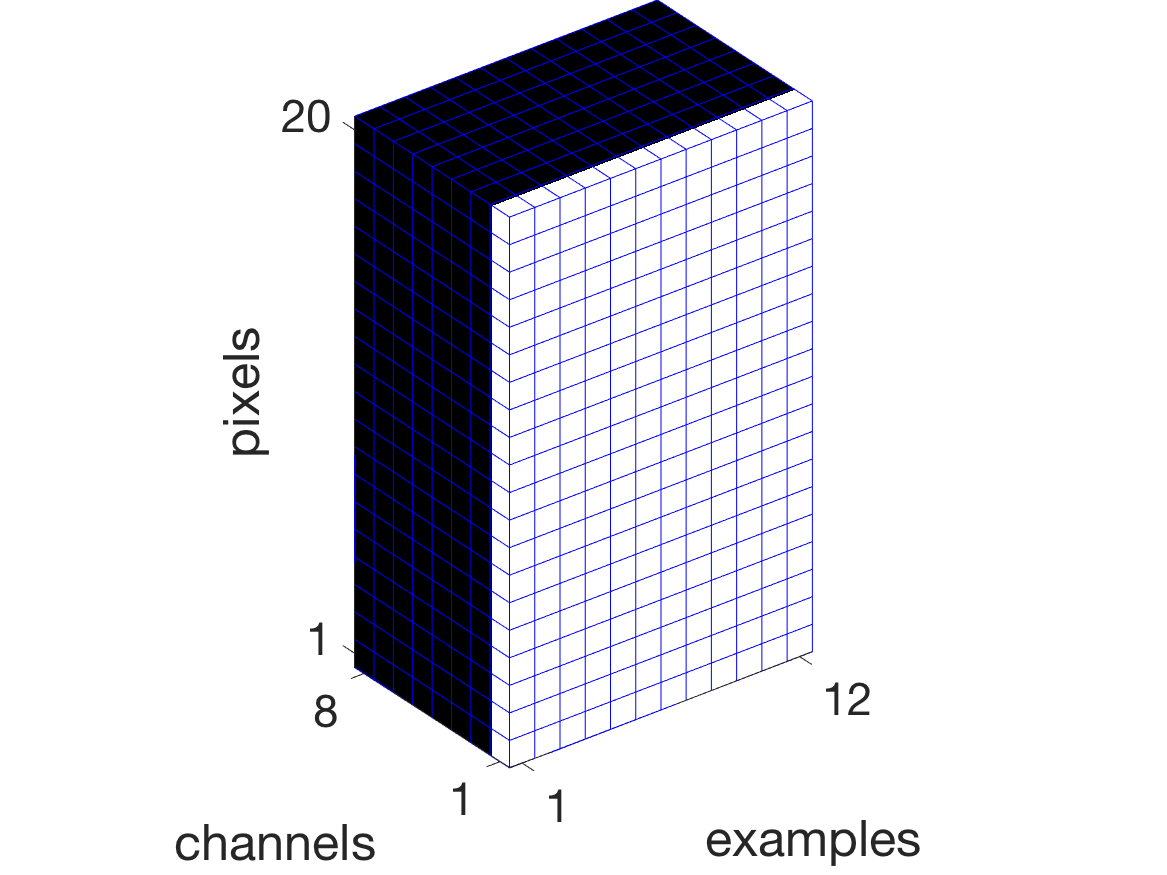
\includegraphics[width=3.5cm]{batchNorm}};
		\node at (.5,0) {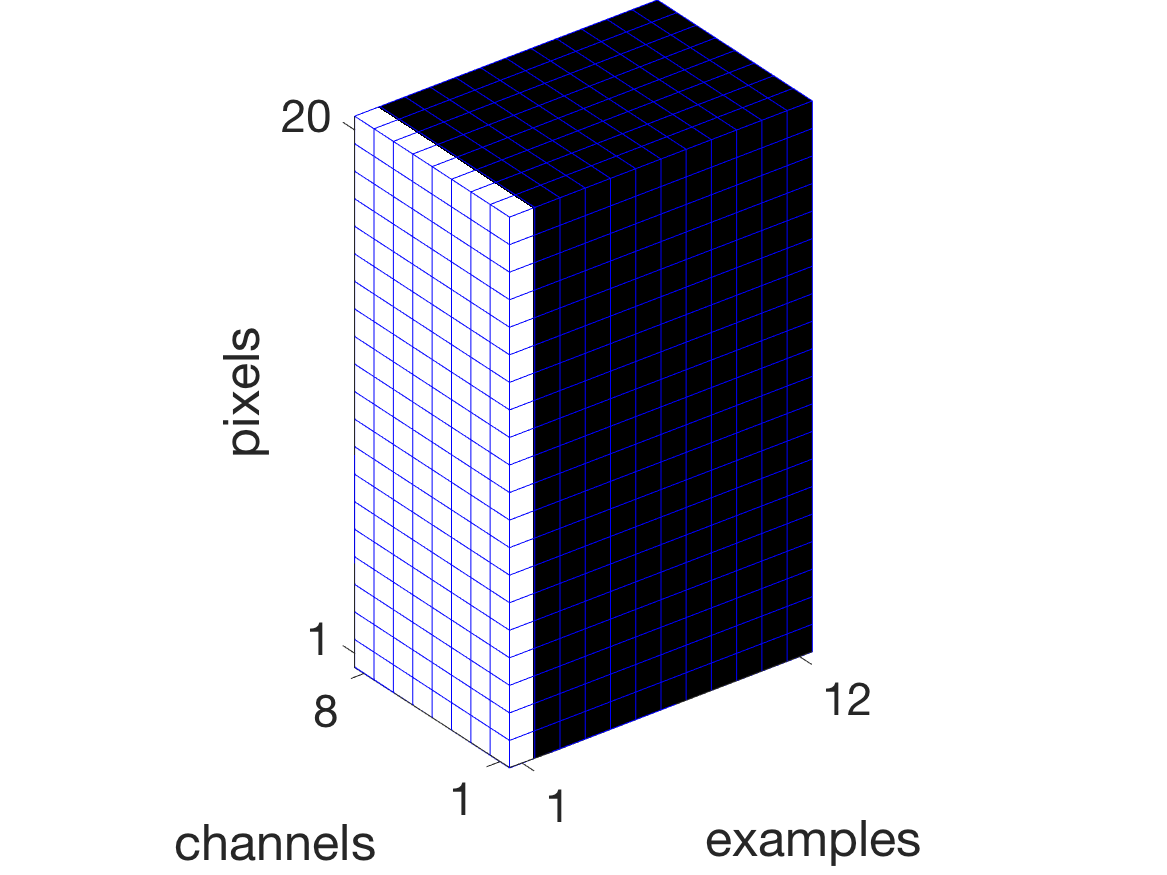
\includegraphics[width=3.5cm]{layerNorm}};
		\node at (3,0) {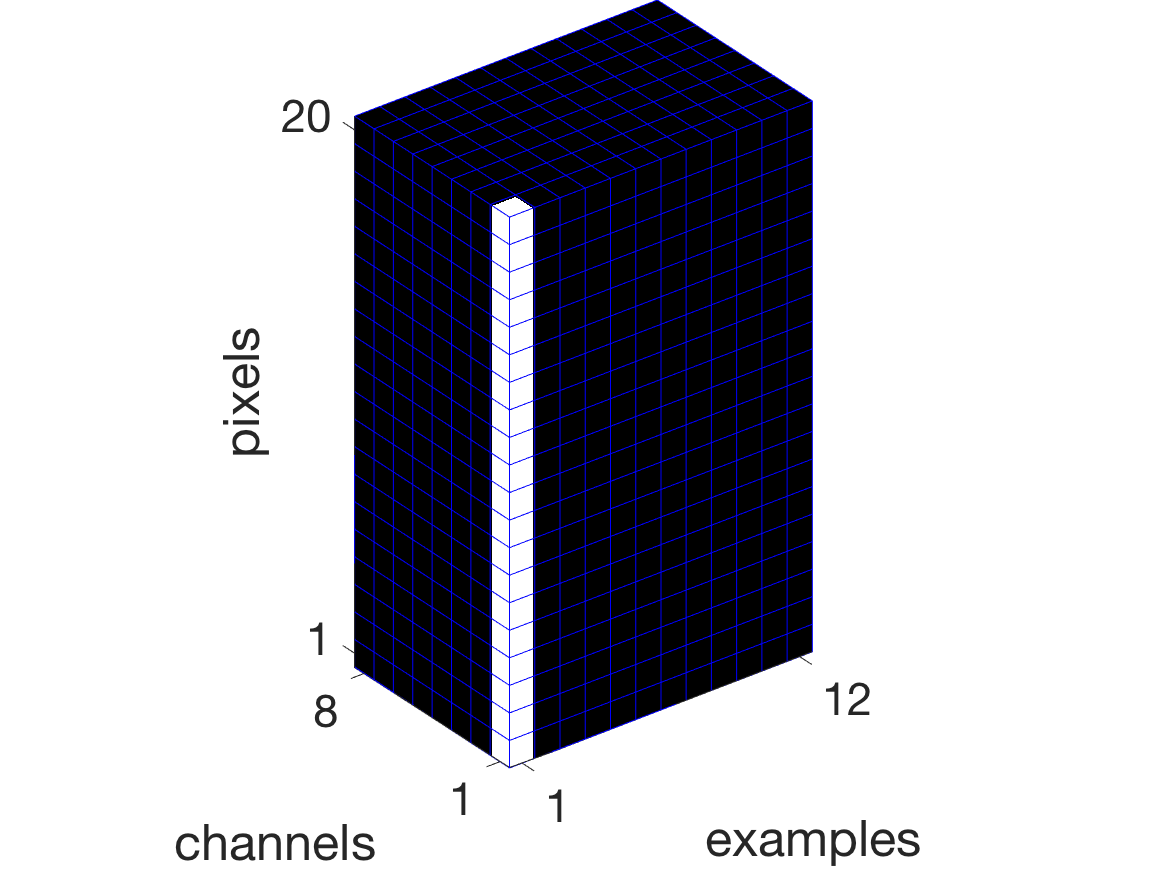
\includegraphics[width=3.5cm]{tvNorm}};
		\node at (5.5,0) {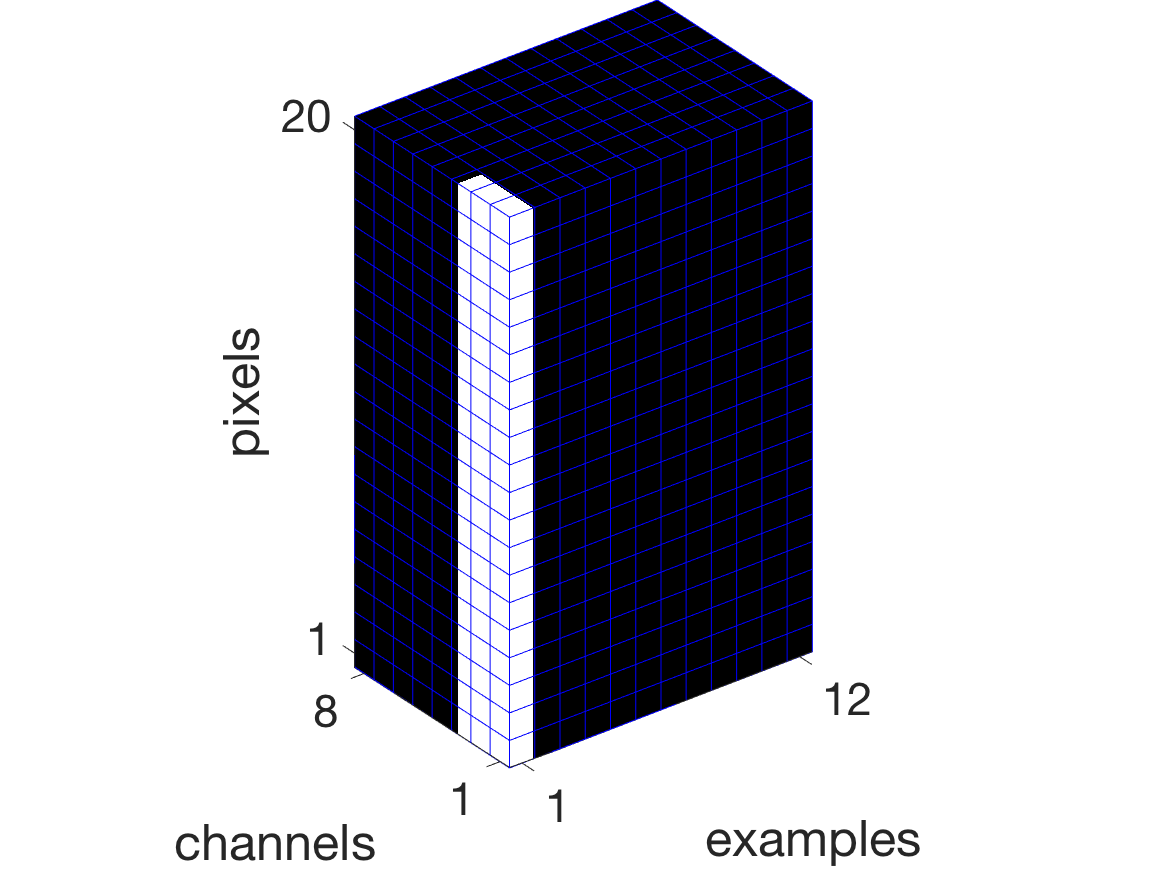
\includegraphics[width=3.5cm]{groupNorm}};
		\node at (-2,1.7) {batch norm};
		\node at (.5,1.7) {layer norm};
		\node at (3,1.7) {instance norm};
		\node at (5.5,1.6) {group norm};
	\end{tikzpicture}
\end{center}

Represent image data as a multidimensional  array
$$ \underbrace{Height\ \times\ Width}_{pixels}\ \times\ Channels\ \times\ Examples $$

We can normalize over each one of those.

\end{frame}

\begin{frame}[fragile]\frametitle{Normalization}

Normalization along \texttt{dir} is done by
\begin{itemize}
\item
Reducing the mean
\begin{verbatim}
	Y = Y - mean(Y,dir)
\end{verbatim}
\item 
Dividing by the standard deviation
\begin{verbatim}
	Y = Y ./ sqrt(Y.^2+eps)
\end{verbatim}
where \texttt{eps}$>0$ is a conditioning parameter.
\end{itemize}

\bigskip
\pause

Questions:
\begin{itemize}
\item How to compute derivatives?

\item The effect of batch size?

\item How well does this work?
\end{itemize}


\end{frame}


\begin{frame}[fragile]\frametitle{Batch Normalization}

\begin{itemize}
\item
the first normalization suggested~\cite{IoffeSzegedy2015}
\item
coupling across examples. Intuitive?

\item sensitive to batch size
\item 
works very well (i.e., better performance of SGD)
\end{itemize}

\bigskip

\begin{center}
	\texttt{E15BatchNorm.m}
\end{center}

\end{frame}

\begin{frame}[fragile]\frametitle{Instance Normalization}

Suggested recently~\cite{UlyanovEtAl2016} but has much older roots

Equivalent to total variation in image denoising~\cite{RudinOsherFatemi1992}

$$TV(\bfY) = {\frac {\grad \bfY}{\sqrt{ |\grad \bfY|^2 + \epsilon}}} $$

Can we utilize this to do better?

\begin{center}
	\texttt{E15InstanceNorm.m}
\end{center}




\end{frame}

\begin{frame}[allowframebreaks]
	\frametitle{References}
\bibliographystyle{abbrv}
\bibliography{NumDNN}

\end{frame}

\end{document}
















